\documentclass[a4paper, 11pt]{article}
\usepackage{graphicx}
\title{Portable Running of Programs for Automation}
\author{G Winter\footnote{g.winter@dl.ac.uk}, 
R. Keegan\footnote{r.m.keegan@dl.ac.uk}, 
CCLRC Daresbury Laboratory}

\begin{document}
\maketitle

\section{Introduction}

Almost any automation in protein crystallography structure solution will 
involve running existing programs at some stage - 
the only alternative is to rewrite 
the substantial body of programs which is available. If we therefore assume 
that running programs is desirable, the only problem is then the matter of 
how.

Some systems, for example autoSHARP [Bricogne et Al., 2002] and 
Elves [Holton \& Alber, 2004], rely on a UNIX shell for this
task - a reliance which has typically been reasonably portable. However, 
in recent years the nature of crystallography and the crystallographer 
has changed - more people are now using Microsoft Windows for ``real''
computing tasks than ever before.

The nature of crystallographic computing is also changing. It used to be 
usual to do all of the computing on a central server - now it's more likely
to be a personal workstation or a cluster of computers. These environments
are both moderately hostile to script based solutions, though can be catered
for.

Here, we describe a more elegant solution, where the running of the program is 
separated from the rest of the system, in such a way as to allow extension
to cover a variety of platforms. Implementation of this system in 
Python\footnote{http://www.python.org} is
also discussed, along with some experiences of using the system in anger.

\section{The Problem}

As described in the introduction, developing a system to automate a protein
crystallography process often depends on interaction with the operating 
system to run programs. This interaction can be difficult to port from 
one platform to another, and can therefore limit the possible users of the 
system.

In general, when running programs for automating a crystallographic process, 
we are interested in the following:

\begin{itemize}
\item{Starting the program}
\item{Providing program input}
\item{Reading program output}
\item{Deciding if the program has worked}
\item{Handling input and output files}
\item{Handling cases where things go wrong, for example killing the program}
\end{itemize}

Of course, almost all systems will interact with more than one program, 
so chaining will be important. This is however out of the scope of this 
discussion. 

Developing portable tools to do this in addition to developing the 
``interesting stuff'' is not a trivial undertaking. 

\section{Conceptual Solution}

Once we have decided on the functionality we want for running programs, 
it is relatively straightforward to design an interface. Given an interface,
the only problem is then to implement or \emph{realize} this interface,
to give us something we can use. The interface described above we call 
``Driver'', and is shown as a UML diagram in 
Figure~\ref{figure:driverinterface}.

\begin{figure}
\centerline{
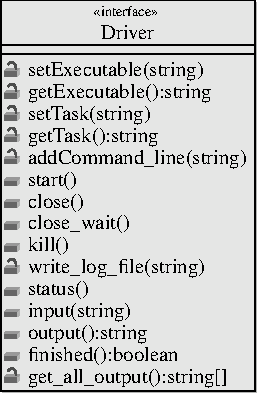
\includegraphics[scale=0.667]{UML/DriverInterface-1.pdf}
}
\caption{The ``Driver'' interface.}
\label{figure:driverinterface}
\end{figure}

Since there are a number of ways we could implement this interface, and a
number of environments where this could take place, the next task is
to design a mechanism to hide these details from the application. A
useful metaphor or pattern\footnote{If you want to find out more about this,
google ``Design Patterns.''} here is the factory. We ask the factory to 
provide something which satisfies the interface Driver, and it provides
such a thing.
This is illustrated in Figure~\ref{figure:driverfactory}. In this way the 
factory can be delegated to provide the most useful implementation for the
current environment.

\begin{figure}
\centerline{
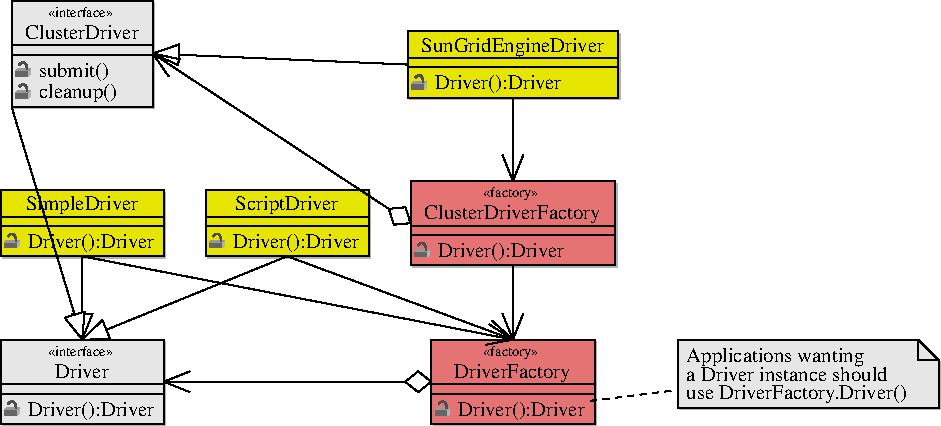
\includegraphics[scale=0.667]{UML/Driver-1.pdf}
}
\caption{Accessing Driver implementations from a factory.}
\label{figure:driverfactory}
\end{figure}

In some cases there will be sets of Driver implementations which have a 
lot in common. For example, batch queuing systems on clusters all work by
submitting  a script. Writing the script and handling the status of the 
job is a general problem, while the details of the submission will depend
on the exact cluster. We can therefore define a new interface, ClusterDriver,
and a new factory to produce them. This factory can then be called by the 
``general'' DriverFactory when a Driver is wanted in a cluster environment.

Although the functionality we want \emph{in general} is described above,
there is often a great deal of commonality between programs in a suite.
For example, in CCP4 most programs accept the ``logical names'' HKLIN, HKLOUT.
We could implement this every time we want to write a program, but this 
will be both untidy and inefficient. A more elegant solution is to take
the Driver instance and ``decorate\footnote{Another design pattern}''
this with the things which are nice for running CCP4 programs, in particular
methods for assigning HKLIN \& HKLOUT files, checking the status and parsing
loggraph output. However, unlike standard inheritance, this must be able
to decorate anything which implements the Driver interface. This is shown
in Figure~\ref{figure:decoratorfactory}.

\begin{figure}
\centerline{
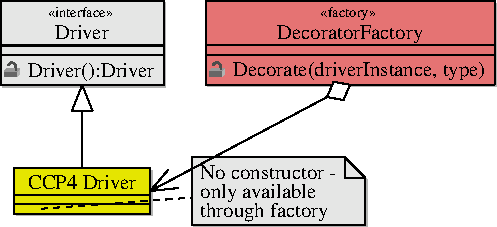
\includegraphics[scale=0.667]{UML/Decorator-1.pdf}
}
\caption{Customizing Driver classes for e.g. CCP4.}
\label{figure:decoratorfactory}
\end{figure}

So far this has involved no programming - we are simply describing a set
of requirements and designing a package which would be able to satisfy those
requirements. What we have described here could be implemented in any 
moderately modern language. In the next section we describe the Python
implementation.

\section{Python Implementation}

Implementing this system in Python is in some ways straightforward, and in 
others rather a challenge. Python includes some very nice tools for interacting
with the operating system, and more often than not these are portable across
the ``usual suspect'' platforms of Linux, Mac OS X and Windows. However,
the language does not include the concept of a virtual class or interface,
as used above. Some interesting ``spells'' were therefore necessary to 
give this kind of functionality. 

Defining the interface is relatively straightforward - simply write a Python
class which looks like what you want, have all of the useful methods raise
exceptions like ``implement me'', and insist that any Driver implementations
inherit from this. A simple check of the class hierarchy can test this.

In python a factory is very simple - this is simply a function which returns
a fresh instance of a class. Implementing the DriverFactory as seen above
therefore only needed one detail - how to specify the default driver type.
This was solved by the old-fashioned approach of setting an environment
variable XIA2CORE\_DRIVERTYPE.

Implementation of the Decorator pattern was less straightforward. Without 
interfaces, a class implementation (lilke CCP4Driver) must inherit from a 
concrete implementation of a Driver class. This presented two possibilities -
either implemnenting $m \times n$ classes like CCP4ScriptDriver, or 
investigating dynamic inheritance. The latter was selected in an instant!

Implementing a system using dynamic inheritance looks a lot like a 
factory function - you have a function that you call which will return 
a new instance of a class. The only difference here is that you pass in 
an instance of the class that you wish to decorate, giving the following
pseudocode:

\begin{verbatim}
function CCP4DriverFactory(DriverInstance d) returns CCP4Driver
{
  DriverClass = d.class()

  class CCP4DecoratorClass(DriverClass)
  {
    // implement class based on Driver interface in here
  }

  return new CCP4DriverClass()
}
\end{verbatim}

In Python, this allows you to decide at construction time what Driver
class we wish to inherit from, and so circumvents the challenges described
above.

This has only one side effect - when you wish to inherit from the
CCP4-decorated driver, you have to have a similar scheme in the code.
However, this ends up being a ten-line boilerplate, which is simply
an empty wrapper which can be populated with the ``interesting stuff''.
This is a relatively small price to pay for portability.

\section{Usage Examples}

\subsection{xia2dpa}

xia2dpa is a toolkit for data processing and analysis, and builds
on the Python implementation of the xia2core described above. This makes 
use of a large number of CCP4 programs as well as programs from outside.
In the new development portability was a key criterion, initiating the 
development of the new core.

xia2dpa is currently being developed in a bottom-up approach. Those components
at the lowest level (program wrappers, inherited from Drivers) are combined
to give useful modules. An example is the development of the xia2scan
application - for analyzing diffraction images when using a humidifier. 
This makes use of 
a couple of ``standard'' programs (labelit.index and labelit.distl
[Sauter et Al., 2004, Zhang et Al, 2006]) and
also makes use of a ``jiffy'' application printheader. All of the programs
have wrappers in the xia2dpa wrapper library, and so can be treated as
functions directly from Python. In this application, results from the indexing
and image analysis are combined to select the best image - from here the 
best humidity for data collection can be selected.

\subsection{MrBUMP}

MrBUMP is a new CCP4 project for doing automated molecular replacement (MR). It is 
implemented in Python and wraps 
around the commonly used MR programs Phaser and Molrep with particular emphasis on
generating search models for use in MR. It takes a brute force approach to the problem
and attempts to generate as many suitable models as is practical. It is designed to
make use of compute clusters to aid this process. Apart from Phaser and Molrep, MrBUMP
makes use of several other CCP4 utility programs for preparing the structure coodinate
files of the search models such as Chainsaw, Pdbcur, PDbset and Coord\_format.

MrBUMP is designed as a framework allowing for additional model preparation methods and
MR programs to be incorporated into it as it is further developed. The ease with which
the xia2core Driver allows for the creation of wrappers to programs is ideal for MrBUMPs
purposes. In addition the built-in portability afforded by xia2core means that program
wrappers can be developed on a single platform and be guaranteed to work on any other
platform. Another particularly attractive feature of the implementation is the Cluster Driver that can
allow MrBUMP to 
take advantage of the wide variety of different clustering systems available such Sun Grid
Engine, PBS, and LSF to name but a few, without having to be tailored to handle the 
idosyncrasies of each of these systems.
 
Currently, MrBUMP has its own built-in wrappers for each of the programs it uses but 
re-writing these to make use of xia2core has proven to be a fairly trivial task given
the simple way in which interfaces can be designed using xia2core. A developer looking
to utilise it only needs a very rudimentary understanding of how the underlying Driver
and Decorator classes are implemented before they can make use of them. This ``low potential
barrier'' to use is perhaps the most appealing feature of xia2core from a practical point of view.     

  

\section{Discussion \& Availability}

\subsection{License}

This software is provided under the CCP4 ``Applications'' license, and
should shortly be distributed as a part of the CCP4 suite, in version 6.1.

\subsection{Download}

The latest version of the xia2core, including the Python implementation
described here, is available from 
http://www.ccp4.ac.uk/xia/xia2core-0.0.3.tar.gz. For information on
more up-to-date versions when available, please contact g.winter@dl.ac.uk.

\section{References}

\begin{itemize}
\item{Bricogne, G., Vonrhein, C., Paciorek, W., Flensburg, C., Schiltz, M., 
Blanc, E., Roversi, P., Morris, R. \& Evans, G. (2002). Acta Cryst. A58, C239.}

\item{Holton, J \& Alber, T, (2004) PNAS 101, 1537-42.}

\item{Sauter, N. K., Grosse-Kunstleve, R. W. \& Adams, P. D. (2004). 
J. Appl. Cryst. 37, 399-409.}

\item{Zhang, Z., Sauter, N. K., van den Bedem, H., Snell, G. \& 
Deacon, A. M. (2006). J. Appl. Cryst. 39, 112-119.}
\end{itemize}


\end{document}
